\documentclass[11pt,letterpaper]{article}
\usepackage[lmargin=1in,rmargin=1in,bmargin=1in,tmargin=1in]{geometry}
\usepackage{quiz}

% -------------------
% Content
% -------------------
\begin{document}
\thispagestyle{title}

% Quiz 1
\quizsol \textit{True/False}: The expression $12 \div 6 \cdot 2 + (-1)^3$ is the same as $\frac{12}{6 \cdot 2} + (-1)^3$ and both are equal to $0$. \pspace

\sol The statement is \textit{false}. We can compute both, following order of operations (PEMDAS, applied carefully left-to-right), and show that the expressions evaluate to different values:
	\[
	\begin{gathered}
	12 \div 6 \cdot 2 + (-1)^3 \\
	12 \div 6 \cdot 2 - 1 \\
	2 \cdot 2 - 1 \\
	4 - 1 \\
	3
	\end{gathered} \hspace{4cm}
	\begin{gathered}
	\tfrac{12}{6 \cdot 2} + (-1)^3 \\
	\tfrac{12}{6 \cdot 2} - 1 \\
	\tfrac{12}{12} - 1 \\
	1 - 1 \\
	0
	\end{gathered}
	\]
For these two expressions to be the same, the first needs a set of parentheses around the $6 \cdot 2$: $12 \div (6 \cdot 2) + (-1)^3$. \pvspace{1.3cm}



% Quiz 2
\quizsol \textit{True/False}: The point $(2, -6)$ is in the third quadrant and is a distance of 2 away from the $x$-axis and a distance of $6$ away from the $y$-axis. \pspace

\sol The statement is \textit{false}. Because $x= 2 > 0$ and $y= -6 < 0$, the point $(2, -6)$ is in Quadrant~IV. Moreover, plotting the point $(2, -6)$, we can see that the point is a distance of $|2|= 2$ away from the $x$-axis and a distance of $|-6|= 6$ away from the $y$-axis. 
	\[
	\fbox{
	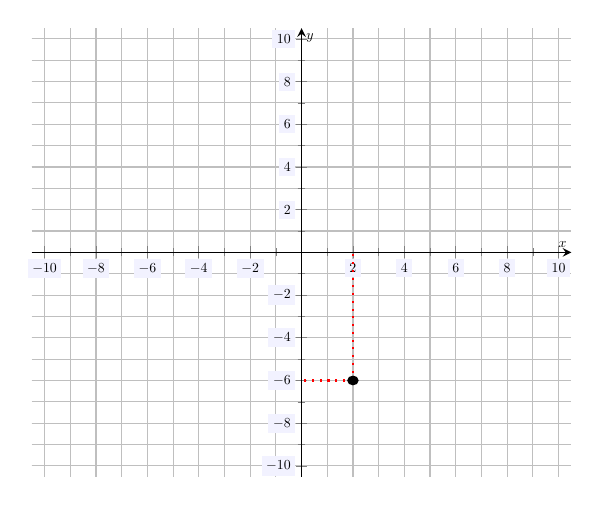
\begin{tikzpicture}[scale=1,every node/.style={scale=0.5}]
	\begin{axis}[
	grid=both,
	axis lines=middle,
	ticklabel style={fill=blue!5!white},
	xmin= -10.5, xmax=10.5,
	ymin= -10.5, ymax=10.5,
	xtick={-10,-8,-6,-4,-2,0,2,4,6,8,10},
	ytick={-10,-8,-6,-4,-2,0,2,4,6,8,10},
	minor tick = {-10,-9,...,10},
	xlabel=\(x\),ylabel=\(y\),
	]
	\draw[dotted,thick,red] (2,-6) -- (0,-6);
	\draw[dotted,thick,red] (2,-6) -- (2,0);
	\draw[fill=black] (2,-6) circle (0.2);
	\end{axis}
	\end{tikzpicture} 
	}
	\] \pvspace{1.3cm}



% Quiz 3
\quizsol \textit{True/False}: The average rate of change of a function is the quotient of the change in output by the change in input. If the average rate of change is positive, the function increased. If the average rate of change is negative, the function decreased. \pspace

\sol The statement is \textit{true}. We know that the average rate of change of a function $f(x)$ over the interval $[a, b]$ is given by $\frac{f(b) - f(a)}{b - a}$. Because $x$'s are the inputs and $f(x)$'s are the outputs, this is $\frac{\Delta \text{output}}{\Delta \text{input}}$. Now because $b > a$, we know that $b - a > 0$. So the sign of the average rate of change depends only on the sign of $f(b) - f(a)$. If $f(b) - f(a) > 0$, then $f(b) > f(a)$. But then the function increased in value from the value at $x= a$ to the value at $x= b$. If $f(b) - f(a) < 0$, then $f(b) < f(a)$. But then the function decreased in value from the value at $x= a$ to the value at $x= b$. Neither imply that the function was increasing or decreasing, respectively, over the \textit{entire} interval $[a, b]$. \pvspace{1.3cm}



% Quiz 4
\quizsol \textit{True/False}: The average rate of change of a function $f(x)$ on an interval $[a, b]$ is the slope of the secant through the points $\big(a, f(a) \big)$ and $\big(b, f(b) \big)$. \pspace

\sol The statement is \textit{true}. We know that the average rate of change of a function $f(x)$ over the interval $[a, b]$ is given by $\frac{f(b) - f(a)}{b - a}$. Given the points $\big(a, f(a) \big)$ and $\big(b, f(b) \big)$, the slope of the line through them is $m= \frac{\Delta y}{\Delta x}=  \frac{f(b) - f(a)}{b - a}$. 
	\[
	\fbox{
	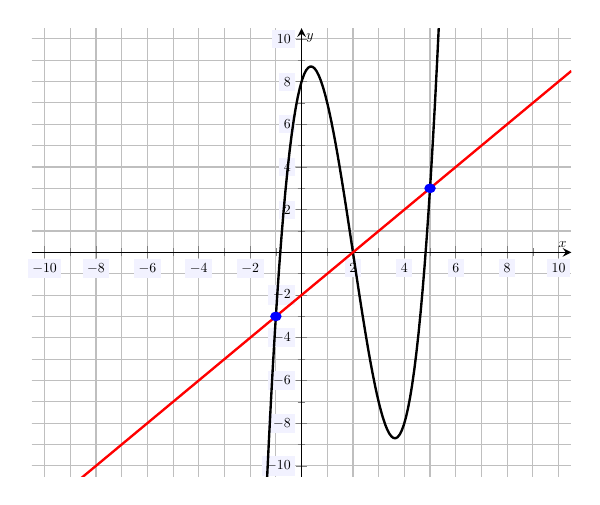
\begin{tikzpicture}[scale=1,every node/.style={scale=0.5}]
	\begin{axis}[
	grid=both,
	axis lines=middle,
	ticklabel style={fill=blue!5!white},
	xmin= -10.5, xmax=10.5,
	ymin= -10.5, ymax=10.5,
	xtick={-10,-8,-6,-4,-2,0,2,4,6,8,10},
	ytick={-10,-8,-6,-4,-2,0,2,4,6,8,10},
	minor tick = {-10,-9,...,10},
	xlabel=\(x\),ylabel=\(y\),
	]
	\addplot[line width=0.03cm, domain= -2:6,samples=100] ({x},{x^3 - 6*x^2 + 4*x + 8});
	\addplot[line width=0.03cm, domain= -9:10.5,samples=2,red] ({x},{x - 2});
	\draw[fill=black,blue] (-1,-3) circle (0.2);
	\draw[fill=black,blue] (5,3) circle (0.2);
	\end{axis}
	\end{tikzpicture} 
	}
	\] \pvspace{1.3cm}



% Quiz 5
\quizsol \textit{True/False}: If $P(t)= 5300t - 1480$ is a linear model representing the population in a small town $t$~years from now, then $m= 5300 > 0$ means that the model says that the population is growing at a rate of 5,300 people per year. Furthermore, the $y$-intercept $b= 1480$ represents the exact initial population of the town. \pspace

\sol The statement is \textit{false}. We know that the function $P(t)$ is linear, i.e. the graph of $P(t)$ is a line. We know that $m= 5300$. Recalling that $m= \frac{\Delta P}{\Delta t}$ and writing $5300= \frac{5300}{1}$, we can see that for every one increase in $t$ results in a 5300 increase in $P$, i.e. the population is growing at a rate of 5,300~people per year. Of course, this is just what the model says happens, on average. The $y$-intercept is $P(0)= 5300(0) - 1480= -1480$. But then $b \neq 1480$. Because $b= P(0)= -1480 < 0$, this cannot possibly represent a population. Furthermore, $b= P(0)$ need not represent the \textit{exact} initial population, merely what the model predicts is the initial population. \pvspace{1.3cm}



% Quiz 6
\quizsol \textit{True/False}: The line $y= 5 - 3x$ and the line through $(0, 5)$ with slope $-3$ must be the same line. \pspace

\sol The statement is \textit{true}. There is a unique line with a specified slope through any point, i.e. all that is needed to determine a line is a point and a slope. The line $y= 5 - 3x$ has slope $-3$. Furthermore, because $5 - 3(0)= 5$, the line $y= 5 - 3x$ contains the point $(0, 5)$. Therefore, these lines must be the same. Alternatively, we can find the line through $(0, 5)$ with slope $-3$ using the point-slope form: $y= y_0 + m(x - x_0)= 5 - 3(x - 0)= 5 - 3x$. One can also use the fact that $(0, 5)$ is a $y$-intercept so that this forces $b= 5$. Because the line has slope $-3$, we must have $y= -3x + 5= 5 - 3x$. In either case, both lines are $y= 5 - 3x$. \pvspace{1.3cm}



% Quiz 7
\quizsol \textit{True/False}: The quadratic function $f(x)= 5 - (x + 6)^2$ opens upwards and has vertex $(6, 5)$. \pspace

\sol The statement is \textit{false}. Recall that the vertex form of a quadratic function is $a(x - P)^2 + Q$, where $a$ is the $a$ from the standard form $ax^2 + bx + c$ and $(P, Q)$ is the vertex. We have $f(x)= 5 - (x + 6)^2= -\big(x - (-6) \big)^2 + 5$. Therefore, $a= -1 < 0$ so that the quadratic function opens downwards. Furthermore, the vertex is $(-6, 5)$. The given solution incorrectly identifies the $a$-value and vertex. \pvspace{1.3cm}



% Quiz 8
\quizsol \textit{True/False}: $\dfrac{2.2 \cdot 10^8}{5.5 \cdot 10^{-3}}= 0.4 \cdot 10^{11}$ \pspace

\sol To compute products and quotients of real numbers in scientific notation, one need compute the product/quotient of the mantissa/significand and the exponential portion and then make an necessary adjustments to the power based on the resulting mantissa/significand. We then have\dots
	\[
	\dfrac{2.2 \cdot 10^8}{5.5 \cdot 10^{-3}}= \dfrac{2.2}{5.5} \cdot \dfrac{10^8}{10^{-3}}= 0.4 \cdot 10^{8 - (-3)}= 0.4 \cdot 10^{11}= 4.0 \cdot 10^{12}
	\] 
The given solution forgets to correctly place the resulting real number in scientific notation by adjusting the power after dividing the mantissas. \pvspace{1.3cm}



% Quiz 9
\quizsol \textit{True/False}: $\dfrac{x^5}{(x^2)^4}= x^{-3}$ \pspace

\sol The statement is \textit{true}. Recall that $x^a x^b= x^{a+b}$, $\frac{x^a}{x^b}= x^{a-b}$, and $(x^a)^b= x^{ab}$. But then\dots
	\[
	\dfrac{x^5}{(x^2)^4}= \dfrac{x^5}{x^8}= x^{-3}
	\]
Of course, $x^{-3}= \frac{1}{x^3}$. \pvspace{1.3cm}



% Quiz 10
\quizsol \textit{True/False}: $\sqrt[5]{x^{10}}= x^{10/5}= x^2$ \pspace

\sol The statement is \textit{true}. Recall that $\sqrt[b]{x^a}= \left( \sqrt[b]{x} \right)^a= x^{a/b}$. But then\dots
	\[
	\sqrt[5]{x^{10}}= x^{10/5}= x^2
	\] \pvspace{1.3cm}



% Quiz 11
\quizsol \textit{True/False}: If $a, b$ are constants, then $f(x)= x^3 + ax + b$ is a polynomial and it is possible for $f(x)$ to have four zeros. \pspace

\sol The statement is \textit{false}. Recall the Fundamental Theorem of Algebra states that a polynomial of degree $n$ has at most $n$ zeros (and exactly $n$ zeros if only allows complex numbers and counts with multiplicity). The degree of $f(x)$ is three. Therefore, it is not possible for $f(x)$ to have four zeros. 


%Factoring $16x^4 - 1$ as completely as possible (using rational numbers) results in the factorization $(4x^2 - 1)(4x^2 + 1)$.


%Let $f(x)$ be a quadratic function. The function $f(x)$ will factor `nicely' if and only if $\text{disc } f(x)$ is a perfect square. 

%The polynomial $2x^2 - 16x + 22$ has roots $4 \pm \sqrt{5}$. Therefore, it factors as $\big(x - (4 - \sqrt{5}) \big) \big(x - (4 + \sqrt{5}) \big)$. 




















\end{document}